\section{问题一：数据质量评价、冲突消解与领域配比模型}
\label{sec:problem1}

问题一的求解分为两条链（图~\ref{fig:p1_flow}）：\textbf{质量链}以文本为单位，完成“指标同向化 $\rightarrow$ 分块赋权 $\rightarrow$ 冲突识别与稳健消解 $\rightarrow$ 领域聚合”；\textbf{配比链}以训练配方为单位，完成“单纯形建模 $\rightarrow$ 响应面选择 $\rightarrow$ 跨规模检验 $\rightarrow$ 支持域内寻优”。两条链在“领域质量是否解释配比收益”处汇合，并向问题二输出基线质量 $Q_0$、参考配比 $\boldsymbol p_{\mathrm{ref}}$ 与配比响应 $R(\boldsymbol p)$。

\begin{figure}[htbp]
\centering
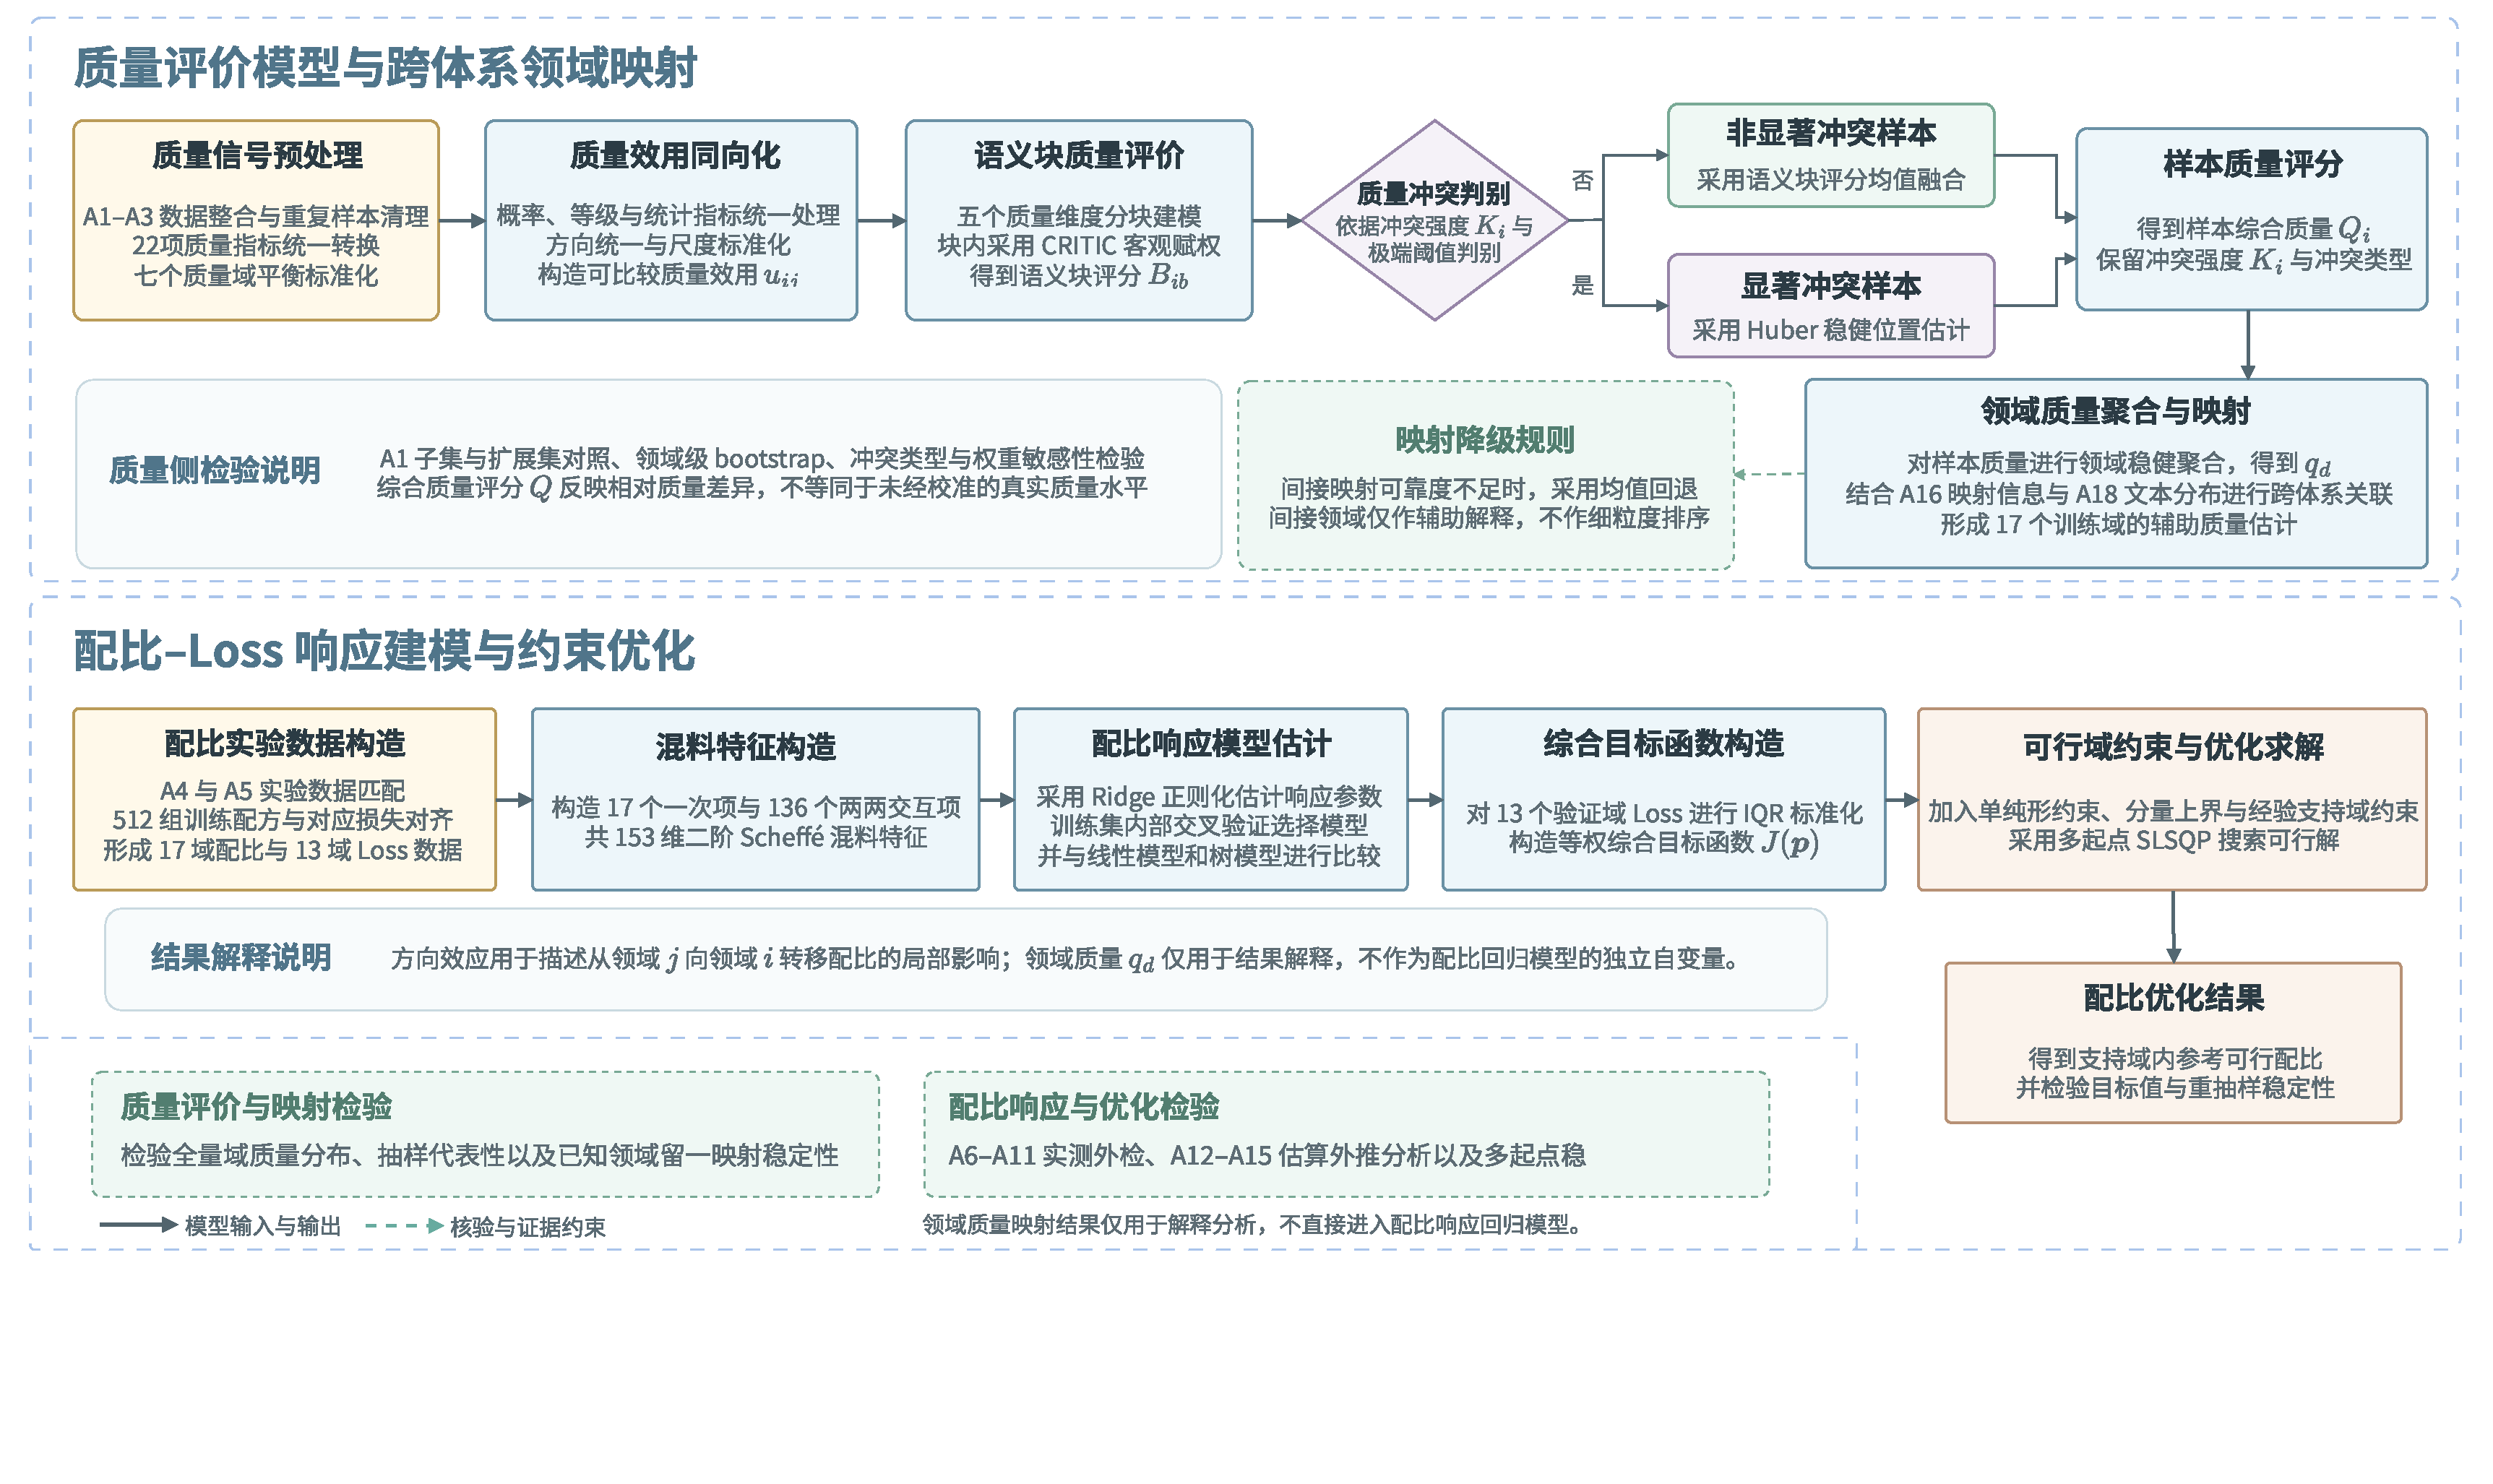
\includegraphics[width=0.97\linewidth]{images/no1/P1_F00R_问题一求解流程图.pdf}
\caption{问题一求解流程：质量评价链与配比建模链}
\label{fig:p1_flow}
\end{figure}

\subsection{数据预处理}

各附件的统计单位与用途见表~\ref{tab:p1_data}。检验集与外推表只在模型冻结后使用一次，不参与模型选择与调参。

\begin{table}[htbp]
\centering
\small
\caption{问题一使用的数据及其用途}
\label{tab:p1_data}
\begin{tabular}{p{0.13\linewidth}p{0.33\linewidth}p{0.45\linewidth}}
\toprule
附件 & 规模 & 用途 \\
\midrule
A1 / A2 / A3 & $51230$ / $17523$ / $203752$ 条质量记录 & 质量评价、冲突分析；A1 为抽样集，A2(arXiv)、A3(GitHub) 为扩展集 \\
A4 / A5 & $512$ 组配方 × 13 个验证域 Loss & 配比响应面训练与五折交叉验证 \\
A6--A11 & 1M、60M 各 $256$ 组，1B $64$ 组 & 冻结模型后的独立检验 \\
A12--A15 & 10B、70B 各 $63$ 组（估算标签） & 外推稳健性讨论 \\
A16 / A18 & 领域映射指引、17 域原始文本样本 & 质量域到配比域的映射 \\
\bottomrule
\end{tabular}
\end{table}

\textbf{去重。}A1 与 A2、A3 分别有 $1419$ 条 arXiv、$10000$ 条 GitHub 记录重合。以“规范化领域名 + 样本 ID”联合去重，重合记录的质量字段逐一核对无冲突，最终得到 $261086$ 条独立记录。少量非有限值（A1 中 18 条、A3 中 1 条）保留为缺失，评分时只用有效指标并在块内重新归一权重，不做均值插补。

\textbf{单纯形闭合。}配比表与 Loss 表按 \texttt{index} 一一配对。存储精度会带来微小的闭合误差，对第 $r$ 组配方作非负截断与重新归一化：
\begin{equation}
p_{ri}=\frac{\max(a_{ri},0)}{\sum_{j=1}^{17}\max(a_{rj},0)},\qquad p_{ri}\ge0,\quad \sum_{i=1}^{17}p_{ri}=1,
\label{eq:p1_closure}
\end{equation}
修正后最大行和误差为 $4.44\times10^{-16}$。

\subsection{质量评价模型}

\subsubsection{指标同向化}

先把列表型与 logits 型指标压缩为标量：二分类 logits 取正类概率，六级分类 logits 取有序期望，QuRating\cite{wettig2024qurating} 的四个分量分别转换后取均值，得到题目要求的 22 项指标。为避免 GitHub 等大样本领域主导经验分布，对需要秩变换的指标 $j$ 先在七个质量域内分别估计经验分布，再等权合成平衡参考分布
\begin{equation}
F_j^{\mathrm{bal}}(x)=\frac17\sum_{d=1}^{7}F_{jd}(x),
\label{eq:p1_bal}
\end{equation}
并按其 $0.5\%$、$99.5\%$ 分位截尾。根据指标语义，采用四类效用函数把所有指标统一为“越高越好”的 $u_{ij}\in[0,1]$：
\begin{equation}
u_{ij}=
\begin{cases}
F_j^{\mathrm{bal}}(x_{ij}), & \text{正向指标（如教育价值、流畅度）},\\[2pt]
1-F_j^{\mathrm{bal}}(x_{ij}), & \text{逆向指标（如广告含量、重复 $n$-gram 比例）},\\[2pt]
\min\{F_j^{\mathrm{bal}}(x_{ij})/0.95,\ 1\}, & \text{饱和型指标（词元熵、独特词比例）},\\[2pt]
\exp\!\left[-(z_{ij}-m_j)^2/(2s_j^2)\right], & \text{适中型指标（文本长度、句数、平均词长）},
\end{cases}
\label{eq:p1_utility}
\end{equation}
其中 $z_{ij}=\log(1+\max\{x_{ij},0\})$，中心 $m_j$ 与稳健尺度 $s_j$ 在“高流畅、低广告、高整洁”的可信样本上按七域平衡方式估计。数字字符比例在 GitHub 中属于正常代码结构，故对代码域取适中型、对其余领域取逆向。已在 $[0,1]$ 内且方向明确的模型概率不再做秩变换，以保留概率间距。

\subsubsection{五语义块与稳定 CRITIC 赋权}

按含义把 22 项指标划分为\textbf{教育价值、表达整洁、推理信息、噪声重复、结构充分}五个语义块（图~\ref{fig:p1_weights}）。块内指标信息高度重叠，例如图书、百科、数学三类相似度的相关系数接近 $1$；若直接等权，同类信息会被重复计入。因此块内采用 CRITIC 客观赋权\cite{diakoulaki1995critic}：设指标 $j$ 的标准差为 $\sigma_j$，与同块指标 $h$ 的 Spearman 相关为 $r_{jh}$，其信息量为
\begin{equation}
C_j=\sigma_j\sum_{h\in\mathcal J_b}\left(1-|r_{jh}|\right).
\label{eq:p1_critic}
\end{equation}
为抑制权重对抽样的敏感性，在每域至多 $10000$ 条的分层样本上做 500 次 bootstrap，计算指标跨领域位置统计量的变异系数 $\mathrm{CV}_j$，得到稳定性修正权重
\begin{equation}
\omega_j=\frac{C_j/(1+\mathrm{CV}_j)}{\sum_{h\in\mathcal J_b}C_h/(1+\mathrm{CV}_h)},\qquad \sum_{j\in\mathcal J_b}\omega_j=1 .
\label{eq:p1_weight}
\end{equation}
块间取等权 $1/5$，使任何语义维度都不会因包含的指标多而获得更大话语权。样本 $i$ 在块 $b$ 上的评分为有效指标的加权平均
\begin{equation}
B_{ib}=\frac{\sum_{j\in\mathcal J_b\cap\mathcal O_i}\omega_ju_{ij}}{\sum_{j\in\mathcal J_b\cap\mathcal O_i}\omega_j},
\label{eq:p1_block}
\end{equation}
$\mathcal O_i$ 为样本 $i$ 的有效指标集合；全部样本均无整块缺失。

\begin{figure}[htbp]
\centering
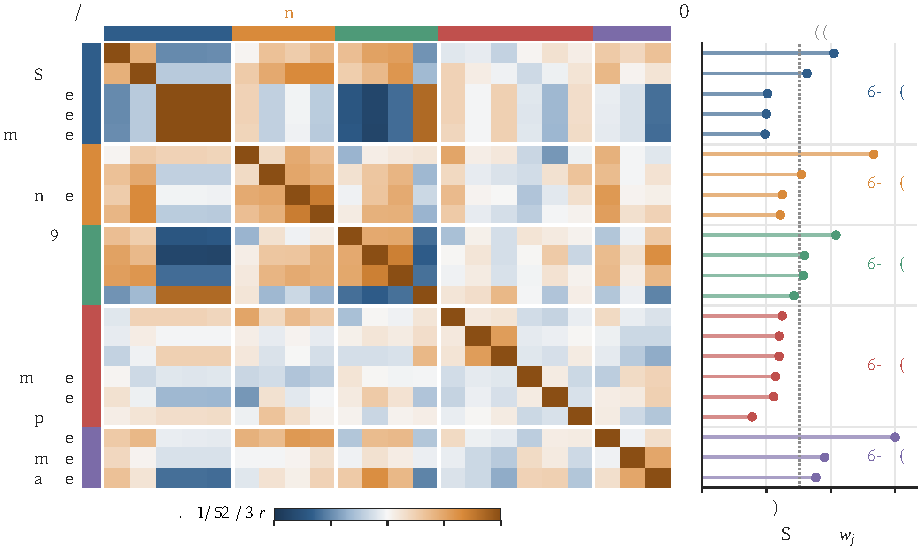
\includegraphics[width=\linewidth]{images/no1/P1_F01_质量指标结构与权重.pdf}
\caption{22 项同向化指标的相关结构（a）与稳定 CRITIC 综合权重（b）}
\label{fig:p1_weights}
\end{figure}

由图~\ref{fig:p1_weights} 可见，指标形成若干明显的相关簇，稳定 CRITIC 自动压低了簇内冗余指标的权重。单项权重最大的平均词长也仅为 $0.090$，终止标点比例、专业性、教育价值分别为 $0.080$、$0.062$、$0.061$，没有任何单一指标主导综合评分。

\subsection{质量冲突的识别与消解}

\subsubsection{冲突的定义}

\begin{definition}[显著质量冲突]
记样本 $i$ 的块间极差 $K_i=\max_bB_{ib}-\min_bB_{ib}$。若同时满足
\begin{equation}
K_i>\mathrm{Q}_{0.90}\left(K\mid d(i)\right),\qquad \max_bB_{ib}\ge0.75,\qquad \min_bB_{ib}\le0.25,
\label{eq:p1_conflict}
\end{equation}
则称样本 $i$ 存在显著质量冲突，其中 $\mathrm{Q}_{0.90}(K\mid d)$ 为所属领域 $d$ 内 $K$ 的 $90\%$ 分位。冲突类型记为“最高块 $>$ 最低块”。
\end{definition}

条件一保证冲突是\textbf{领域内相对}罕见的，避免把代码、论文等领域天然的指标差异误判为冲突；条件二、三保证冲突是\textbf{绝对}显著的，即确有一个维度“很好”而另一个维度“很差”。

\subsubsection{消解规则：Huber 稳健聚合}

对非冲突样本，块间等权平均即可；对冲突样本，简单平均会被极端块拉偏，因此采用 Huber 位置估计\cite{huber1964robust}：
\begin{equation}
Q_i=
\begin{cases}
\dfrac1{|\mathcal B_i|}\displaystyle\sum_{b\in\mathcal B_i}B_{ib}, & i\notin\mathcal C,\\[10pt]
\displaystyle\arg\min_{q\in[0,1]}\sum_{b\in\mathcal B_i}\rho_{1.345}\!\left(\frac{B_{ib}-q}{s_{d(i),b}}\right), & i\in\mathcal C,
\end{cases}
\label{eq:p1_Q}
\end{equation}
其中 $\mathcal C$ 为冲突样本集，$s_{d,b}$ 为领域 $d$ 中块 $b$ 的 MAD 稳健尺度，$\rho_c$ 为 Huber 损失（$|t|\le c$ 时取 $t^2/2$，否则取 $c|t|-c^2/2$）。Huber 估计对“多数块一致、个别块离群”的情形自动降低离群块的权重，但\textbf{不删除任何信息}：冲突强度 $K_i$ 与冲突类型作为附加标签保留。所有冲突样本的 IRLS 迭代均收敛。

\subsubsection{冲突结构与成因}

在 $261086$ 条记录中，显著冲突率为 $3.17\%$（$8270$ 条）。图~\ref{fig:p1_conflict} 给出冲突的领域分布与块对结构，主要发现如下。

\begin{figure}[htbp]
\centering
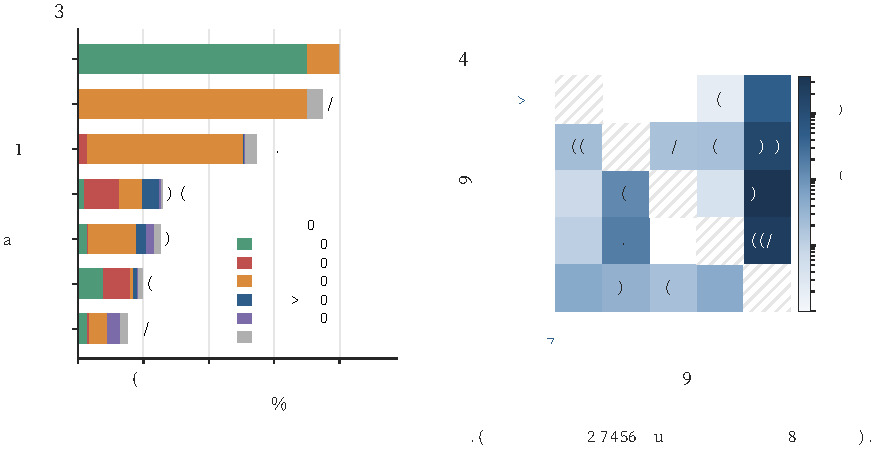
\includegraphics[width=\linewidth]{images/no1/P1_F04_质量冲突机制与稳健消解.pdf}
\caption{质量冲突的领域分布与类型构成（a），以及“高分块 $\rightarrow$ 低分块”冲突计数（b）}
\label{fig:p1_conflict}
\end{figure}

\begin{enumerate}
\item \textbf{冲突几乎全部指向“结构充分”块。}在全部冲突中，低分块为结构充分的占 $93.4\%$，其中“推理信息高—结构充分低”$3640$ 条、“噪声重复（即干净）高—结构充分低”$2290$ 条、“表达整洁高—结构充分低”$1353$ 条。
\item \textbf{成因是“形式指标”与“内容指标”测量对象不同。}结构块由文本长度、句数、平均词长构成，刻画的是篇幅形式；推理、教育、表达等块刻画的是内容。arXiv 片段中大量公式与符号使平均词长和句子切分偏离自然语言中心，形成“推理高—结构低”（占该域冲突的 $87.7\%$）；C4 网页多为短小但行文规范的段落，形成“表达高—结构低”（$91.2\%$）；代码文本重复少、噪声低，但行与“句”的结构不符合自然语言规律，形成“噪声低—结构低”（$42.1\%$）。
\item \textbf{消解是局部的。}Huber 修正对 $252816$ 个非冲突样本为零；对 $8270$ 个冲突样本，修正量均值 $0.077$、中位数 $0.038$。即稳健聚合只调整内部矛盾的样本，不改变整体评分基线。
\end{enumerate}

\textbf{扩展集检验。}arXiv 与 GitHub 两域的记录绝大部分来自扩展集 A2、A3（分别占 $91.9\%$ 与 $95.1\%$）。在这两个以扩展集为主体的领域中，上述结论同样成立：冲突的低分块全部或绝大部分为结构充分块（arXiv 为 $100\%$，GitHub 为 $93.0\%$）；冲突率分别为 $10.00\%$ 和 $2.45\%$，与“公式密集文本冲突多、代码文本冲突少”的成因解释相符。

\subsection{领域质量评价与抽样集对照}

\subsubsection{领域聚合}

样本质量 $Q_i$ 的取值范围为 $[0.141,0.880]$。对领域 $d$，取领域内 $Q_i$ 的 Huber 稳健均值作为领域质量
\begin{equation}
q_d=\arg\min_q\sum_{i\in\mathcal S_d}\rho_{1.345}\!\left(\frac{Q_i-q}{s_d}\right),
\label{eq:p1_qd}
\end{equation}
它介于均值与中位数之间，既不被少量极端样本左右，又比中位数更有效率；并以领域内 500 次 bootstrap 的 $2.5\%$、$97.5\%$ 分位作为区间。结果见表~\ref{tab:p1_quality} 与图~\ref{fig:p1_quality}(a)。

\begin{table}[htbp]
\centering
\small
\caption{七个质量域的领域质量 $q_d$ 与冲突率（全量去重数据）}
\label{tab:p1_quality}
\begin{tabular}{lrcccr}
\toprule
领域 & 样本数 & $q_d$ & 95\% 区间 & 中位数 & 冲突率/\% \\
\midrule
C4 网页 & 10000 & 0.6192 & [0.6173, 0.6210] & 0.6201 & 6.83 \\
通用网页（CommonCrawl） & 9640 & 0.6083 & [0.6067, 0.6097] & 0.6106 & 1.88 \\
学术论文（arXiv） & 17523 & 0.5688 & [0.5679, 0.5697] & 0.5663 & 10.00 \\
技术问答（StackExchange） & 10000 & 0.5608 & [0.5591, 0.5624] & 0.5612 & 3.14 \\
图书（Book） & 171 & 0.5100 & [0.4995, 0.5215] & 0.5134 & 9.36 \\
百科（Wikipedia） & 10000 & 0.5067 & [0.5047, 0.5084] & 0.5038 & 3.22 \\
代码（GitHub） & 203752 & 0.4304 & [0.4301, 0.4306] & 0.4296 & 2.45 \\
\bottomrule
\end{tabular}
\end{table}

C4 与 CommonCrawl 质量最高——二者本身就是经过规则过滤的网页语料\cite{penedo2024fineweb}；GitHub 最低，这是因为多数质量指标（教育价值、流畅度、可读性）面向自然语言设计，代码天然处于劣势。该排序反映的是本指标体系下的相对质量，并非对代码数据训练价值的否定。

\begin{figure}[htbp]
\centering
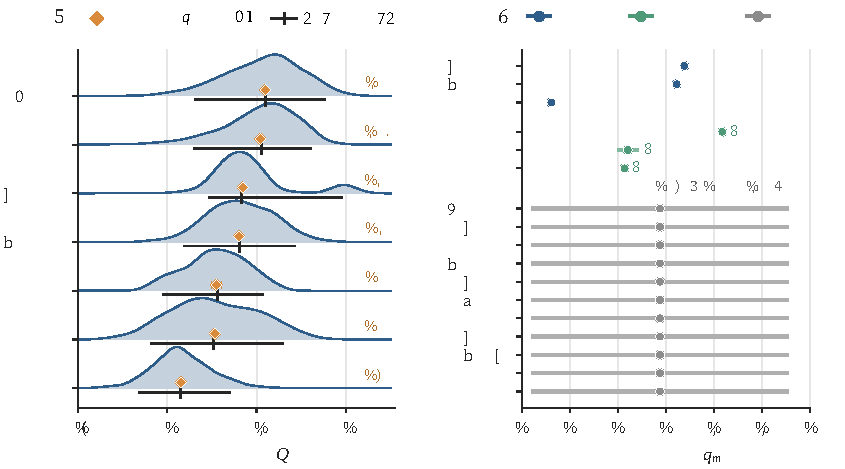
\includegraphics[width=\linewidth]{images/no1/P1_F02_领域质量景观与映射.pdf}
\caption{七个质量域的质量分布（a）与 17 个配比域的映射质量（b）}
\label{fig:p1_quality}
\end{figure}

\subsubsection{全量结果与抽样集 A1 的对照}

题目要求将基于全量记录的域级 $Q$ 与抽样集结果对照。扩展集只覆盖 arXiv 与 GitHub 两域，因此在这两域上比较 A1 抽样记录与扩展集余集（去重后不在 A1 中的记录）的质量分布，见表~\ref{tab:p1_a1_compare} 与图~\ref{fig:p1_repr}。

\begin{table}[htbp]
\centering
\small
\caption{A1 抽样集与扩展集余集的质量分位数对照}
\label{tab:p1_a1_compare}
\begin{tabular}{llccccccc}
\toprule
领域 & 数据 & 样本数 & $P_{10}$ & $P_{25}$ & $P_{50}$ & $P_{75}$ & $P_{90}$ & KS 距离 \\
\midrule
\multirow{2}{*}{arXiv} & A1 抽样集 & 1419 & 0.5090 & 0.5356 & 0.5664 & 0.6057 & 0.6752 & \multirow{2}{*}{0.025} \\
 & 扩展集余集 & 16104 & 0.5076 & 0.5340 & 0.5663 & 0.6024 & 0.7519 & \\
\midrule
\multirow{2}{*}{GitHub} & A1 抽样集 & 10000 & 0.3571 & 0.3927 & 0.4310 & 0.4696 & 0.5103 & \multirow{2}{*}{0.011} \\
 & 扩展集余集 & 193752 & 0.3566 & 0.3916 & 0.4295 & 0.4691 & 0.5101 & \\
\bottomrule
\end{tabular}
\end{table}

两域的主体分位数几乎重合：中位数差分别仅为 $0.0001$ 和 $0.0015$，KS 距离为 $0.025$ 和 $0.011$，Wasserstein 距离为 $0.0029$ 和 $0.0011$，Huber 均值差的 bootstrap 区间均包含 $0$。因此\textbf{基于抽样集与基于全量数据得到的域级质量结论一致}。唯一值得注意的差异出现在 arXiv 的高分尾部：arXiv 质量分布在 $0.78$ 附近有一个次高峰，扩展集余集更早进入该峰，使 $P_{90}$ 处的位移达到 $0.077$（bootstrap 区间 $[-0.052,0.122]$，仍包含 0）。样本量仅 1419 的 A1 对高分尾部的刻画精度有限，这也是本文坚持用全量记录计算域级 $Q$ 的原因。

\begin{figure}[htbp]
\centering
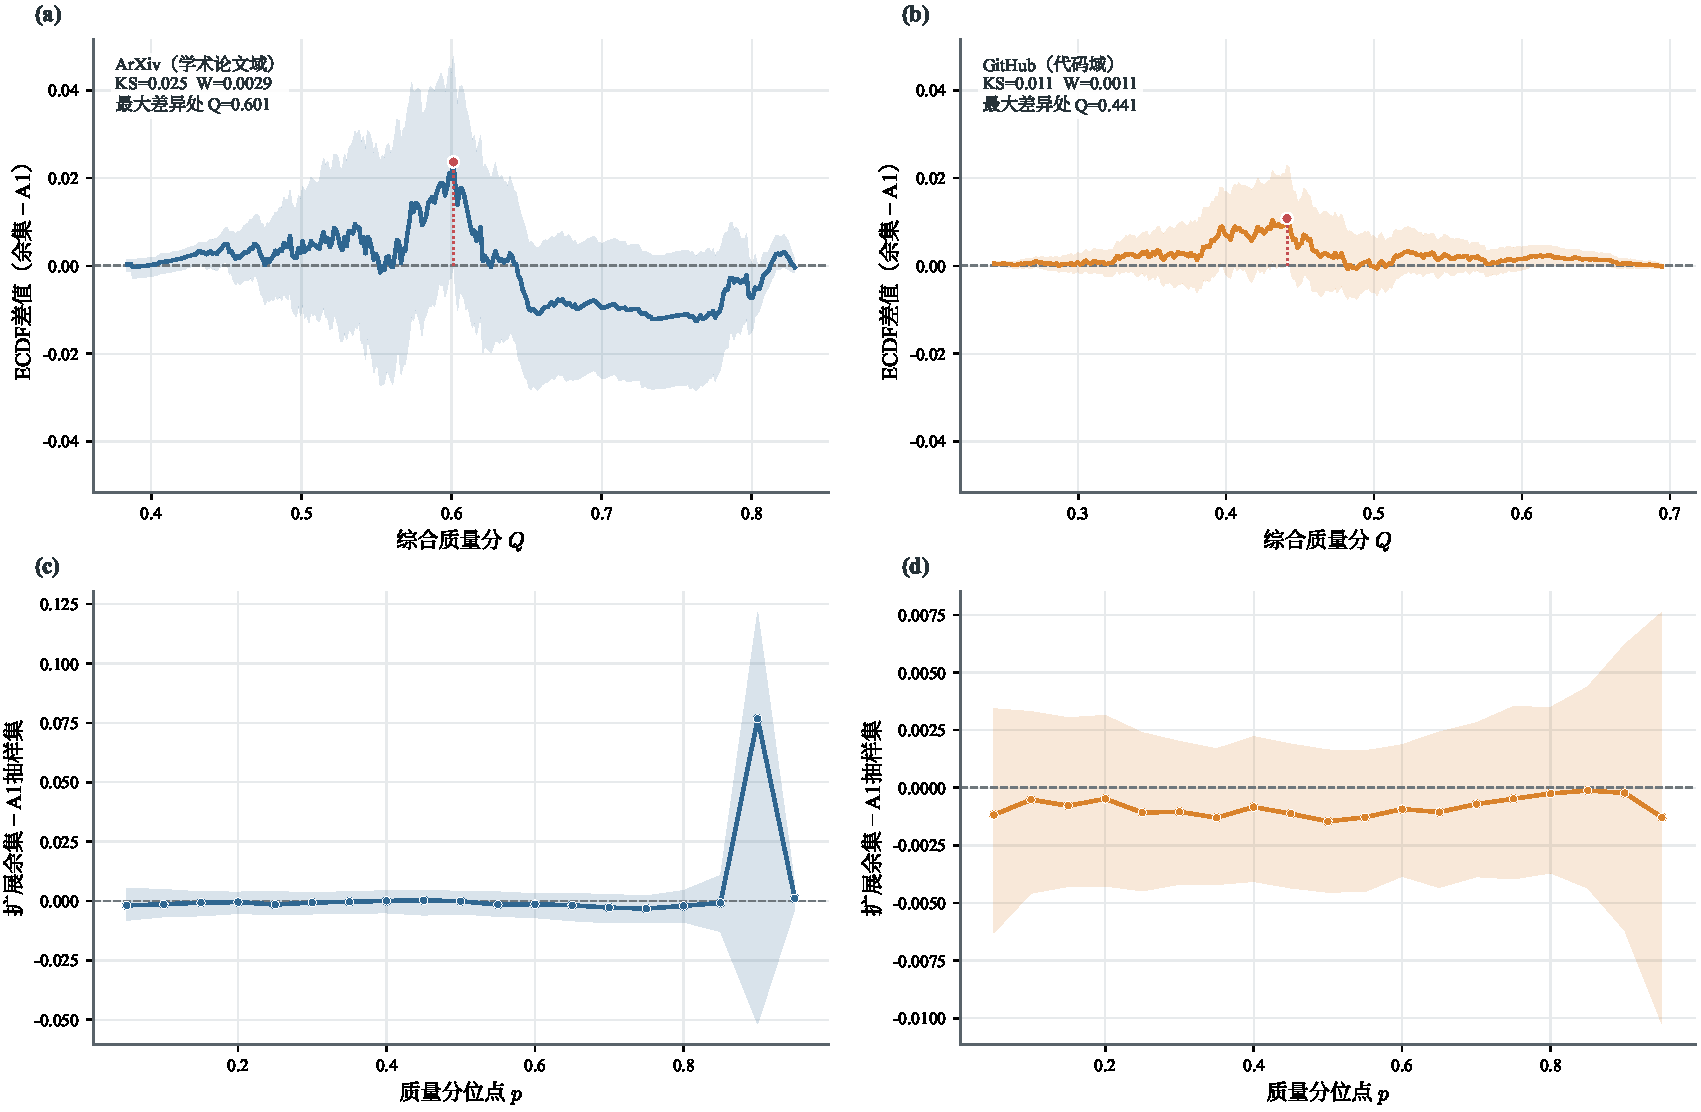
\includegraphics[width=\linewidth]{images/no1/P1_F03_扩展集代表性诊断.pdf}
\caption{A1 抽样集与扩展集余集的分布对照（a）及分位数位移函数（b）}
\label{fig:p1_repr}
\end{figure}

\subsubsection{评分可靠性检验}

从三个角度检验评分的可靠性。

\textbf{（1）聚合规则扰动。}不重新调参，分别改用指标等权、块内等权、取消 Huber、块中位数四种方案。七域排序与主方案的 Kendall 系数最低为 $0.810$，说明领域层面的质量排序稳健；但样本高、低质量极端组的最低重合率为 $0.613$，说明单个文本的精细排名对融合规则更敏感。因此本文把领域级 $q_d$ 作为后续建模的主要输入，而不直接使用样本级排名。

\textbf{（2）原始文本检验。}回到 A1 原始文本，按领域取 $Q_i$ 的最高 $10\%$ 与最低 $10\%$ 两组，比较不依赖任何质量指标的五项文本特征：控制/替换字符率、HTML 与脚本密度、纯 URL 行比例、重复行比例、超长 Token 比例。若评分可靠，高质量组的这五项“脏数据”特征应系统性地低于低质量组。\todo{运行 \texttt{问题一/problem1.py all} 后，将 \texttt{results\_p12\_final\_v2/text\_proxy\_validation.csv} 中各领域 high\_minus\_low 的结果填入此处（建议列成一张 7 域 × 5 特征的小表），并据符号给出结论}

\textbf{（3）与外部认知一致。}C4、CommonCrawl 质量最高、代码最低，与 FineWeb 等工作中“经规则过滤的网页语料教育价值较高”的结论一致\cite{penedo2024fineweb,longpre2024pretrainers}；arXiv 冲突率最高，也与公式文本难以被自然语言指标刻画的常识一致。

\subsubsection{质量向 17 个配比域的映射}

质量数据有 7 个领域，配比实验有 17 个 The Pile 领域\cite{gao2020pile}。参照 A16，3 个领域直接映射（arXiv、GitHub、StackExchange），3 个近直接映射（Pile-CC$\to$CommonCrawl、Wikipedia(en)$\to$Wikipedia、Gutenberg$\to$Book）。其余 11 个领域用 A18 原始文本的长度、字符、结构与重复特征计算其到 7 个锚点的标准化距离 $d_{md}$，按温度 $\tau$ 的软最近邻加权并向公共均值 $\bar q$ 收缩：
\begin{equation}
w_{md}=\frac{\exp[-(d_{md}-d_{m,\min})/\tau]}{\sum_{h=1}^{7}\exp[-(d_{mh}-d_{m,\min})/\tau]},\qquad
q_m=\lambda_m\sum_{d=1}^{7}w_{md}q_d+(1-\lambda_m)\bar q .
\label{eq:p1_map}
\end{equation}
$\tau$ 只由已知域的留一误差选择（$\tau=5$，留一 MAE $=0.057$）。但留一排序的 Spearman 系数为 $-1$，说明文本表层特征\textbf{不能}可靠地区分推断域的质量高低；按照预设规则，11 个推断域的收缩系数 $\lambda_m$ 取 $0$，统一取公共参考质量 $\bar q=0.5435$（bootstrap 区间 $[0.5419,0.5451]$），如图~\ref{fig:p1_quality}(b)所示。这一处理不会低估质量的作用：配比对 Loss 的影响在配比模型中由实验数据直接估计，质量映射只用于构造基线质量 $Q_0$。

\subsection{领域配比—Loss 响应模型}

\subsubsection{Scheff\'e 混料模型}

17 个份额满足式~\eqref{eq:p1_closure} 的单纯形约束，属于组成数据\cite{aitchison1982statistical}。含截距的普通多项式回归会因 $\sum_ip_i=1$ 产生完全共线。Scheff\'e 正则多项式\cite{scheffe1958mixtures,cornell2002mixtures}去掉截距与平方项，把约束直接吸收进模型结构。对第 $k$ 个验证域，
\begin{equation}
\widehat L_k(\boldsymbol p)=\sum_{i=1}^{17}\beta_{ik}p_i+\sum_{1\le i<j\le17}\beta_{ijk}p_ip_j,\qquad k=1,\ldots,13 .
\label{eq:p1_scheffe}
\end{equation}
一次项 $\beta_{ik}$ 是“纯领域 $i$ 训练”时的预测 Loss；交互项 $\beta_{ijk}<0$ 表示领域 $i,j$ 同时出现时 Loss 低于线性混合，即二者\textbf{互补}，$\beta_{ijk}>0$ 则表示\textbf{替代}（或冗余）。模型共 $17+136=153$ 个特征，而训练配方只有 512 组，因此对 13 个验证域联合做多输出 Ridge 估计\cite{hoerl1970ridge}：
\begin{equation}
\widehat{\boldsymbol B}=\arg\min_{\boldsymbol B}\left\|\boldsymbol Y-\boldsymbol X_s\boldsymbol B\right\|_F^2+\lambda\left\|\boldsymbol B\right\|_F^2,
\label{eq:p1_ridge}
\end{equation}
其中 $\boldsymbol X_s$ 为按训练折均方根尺度标准化的 Scheff\'e 设计矩阵，$\boldsymbol Y\in\mathbb R^{512\times13}$。

质量是否需要单独进入该模型？若加入配比加权质量 $\sum_ip_iq_i$，它是一次项的线性组合，与 Scheff\'e 一次项完全共线，无法从配比实验中识别。因此\textbf{领域质量的作用已被一次项吸收}，不单独入模；质量对 Loss 的独立作用在问题二中由附件 B 的质量实验识别。

\subsubsection{模型选择}

在 A4/A5 内按配比结构分层做五折交叉验证，标准化只在训练折内估计，以 13 个验证域的 IQR 标准化 RMSE（NRMSE）为主准则。候选模型比较见图~\ref{fig:p1_select}：二阶 Ridge 的 NRMSE 最低（$0.3959$），优于 Elastic Net（$0.3986$）、线性 Ridge（$0.4108$）、Extra Trees（$0.4307$）与随机森林（$0.4423$）。Extra Trees 的秩相关略高（中位 Spearman $0.8545$ 对 $0.8285$），二者共同构成“误差—排序”Pareto 前沿；二阶 Ridge 在误差上占优，并且是连续可微的显式多项式，可以直接用于梯度分析和约束寻优，故选为主模型。正则化路径显示最优 $\alpha^*=0.0562$ 附近存在 NRMSE 与最优值相差不超过 $1\%$ 的宽平台 $[0.0018,0.178]$，选择并非由单个网格点偶然决定。

\begin{figure}[htbp]
\centering
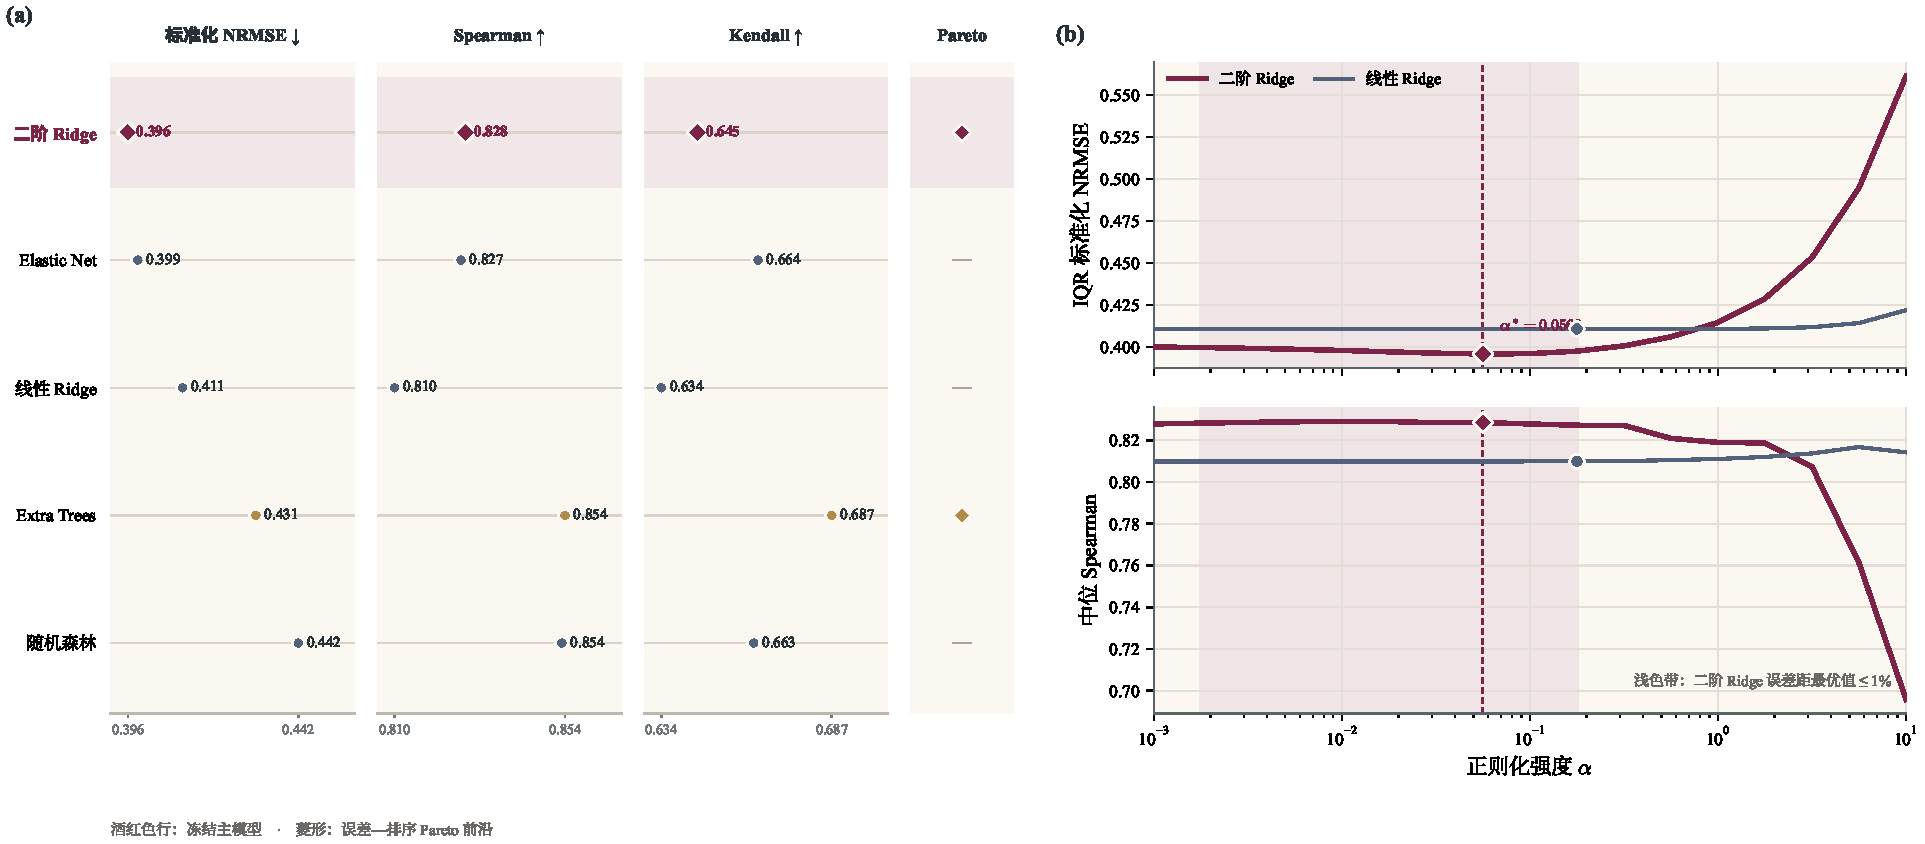
\includegraphics[width=\linewidth]{images/no1/P1_F09_响应面选择与正则化诊断.pdf}
\caption{配比响应模型的交叉验证选择（a）与 Ridge 正则化路径（b）}
\label{fig:p1_select}
\end{figure}

\subsection{配比模型的求解结果}

\subsubsection{检验集验证与外推稳健性}

模型选定后冻结，一次性作用于 A6--A15，结果见表~\ref{tab:p1_test} 与图~\ref{fig:p1_test}。

\begin{table}[htbp]
\centering
\small
\caption{配比响应模型在检验集与外推表上的表现（13 个验证域的中位数）}
\label{tab:p1_test}
\begin{tabular}{llcccc}
\toprule
数据 & 性质 & Spearman & Kendall & $R^2$ & 归一化后悔值 \\
\midrule
A6/A7（1M） & 实测，同规模新配方 & 0.858 & 0.666 & 0.637 & 0.188 \\
A8/A9（60M） & 实测，跨规模 & 0.870 & 0.683 & 0.675 & 0.140 \\
A10/A11（1B） & 实测，跨规模新配方 & 0.850 & 0.688 & 0.324 & 0.061 \\
A12/A13（10B） & 估算标签 & 0.540 & 0.381 & $-231.4$ & 0.743 \\
A14/A15（70B） & 估算标签 & 0.394 & 0.258 & $-373.5$ & 0.806 \\
\bottomrule
\end{tabular}
\end{table}

\begin{figure}[htbp]
\centering
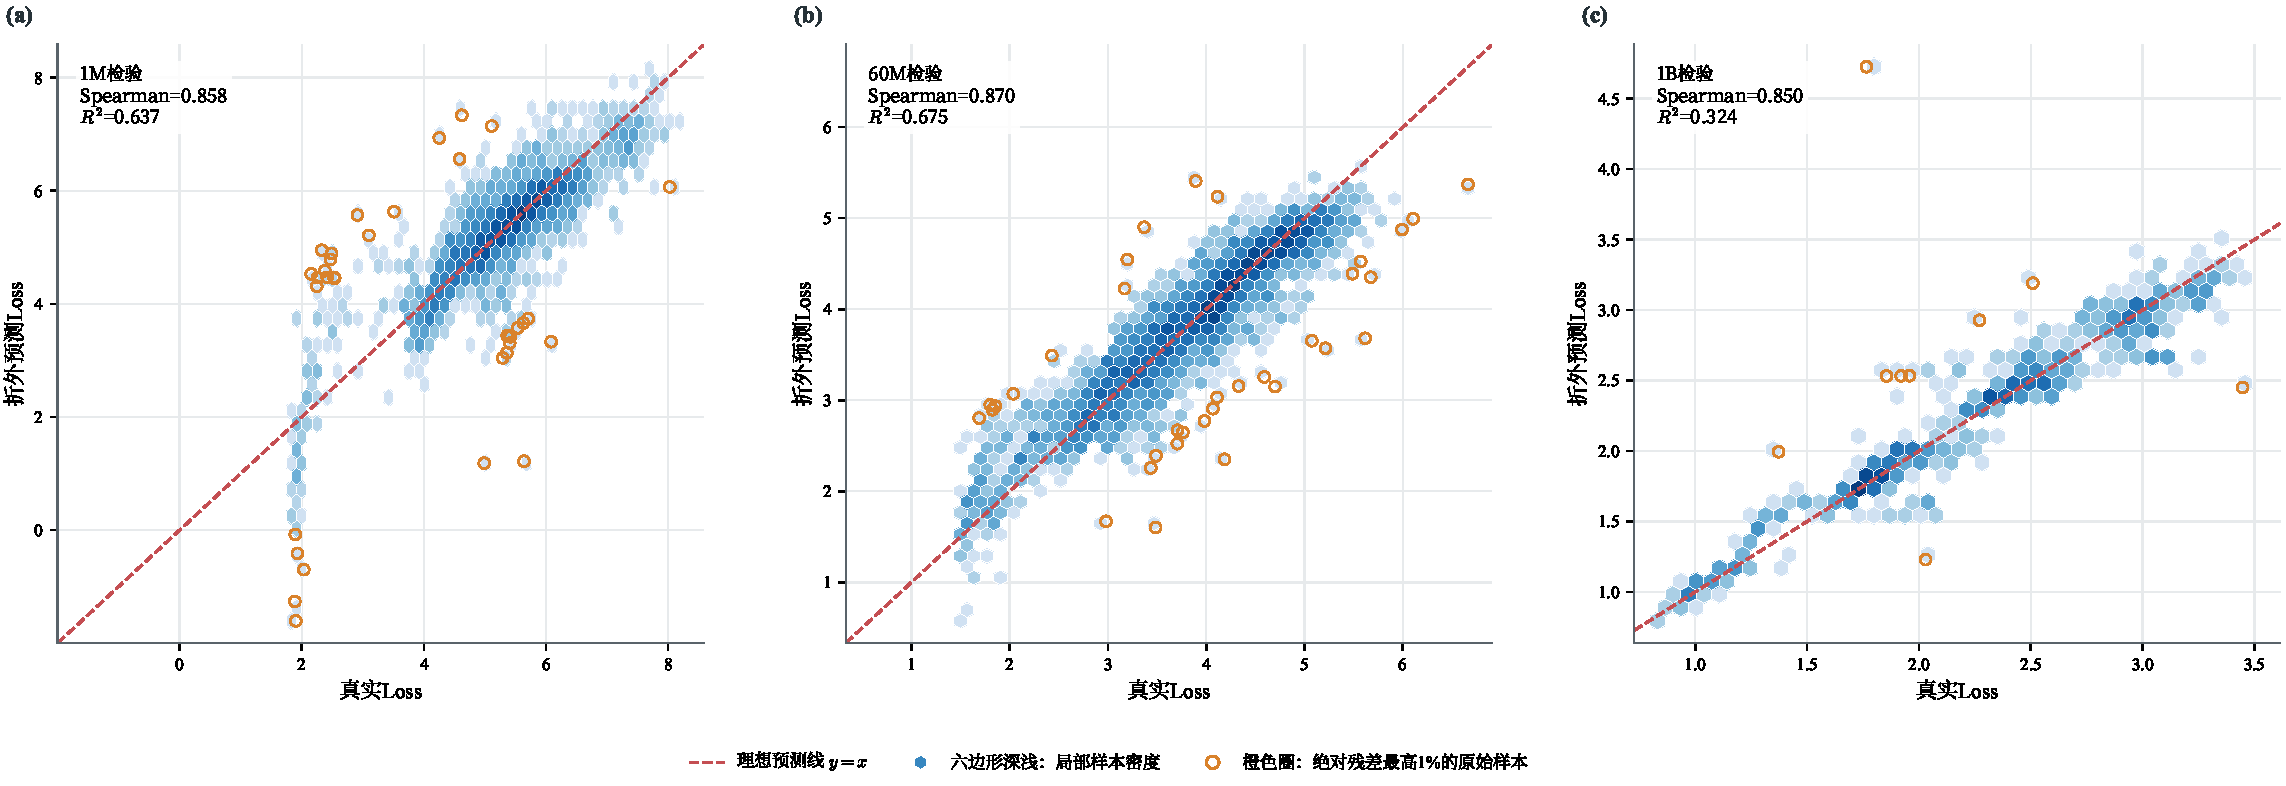
\includegraphics[width=\linewidth]{images/no1/P1_F05_配比模型跨尺度验证.pdf}
\caption{1M、60M、1B 三个实测检验集上的预测 Loss 与真实 Loss}
\label{fig:p1_test}
\end{figure}

三点结论：\textbf{第一}，在三个实测检验集上 Spearman 系数稳定在 $0.85$--$0.87$，说明 1M 规模上学到的配比响应能够跨越三个数量级（1M$\to$1B）保持配方的\textbf{相对优劣}；归一化后悔值随规模增大而下降（$0.188\to0.061$），即按模型选出的配方与真实最优配方的差距越来越小。\textbf{第二}，1B 上 $R^2$ 降至 $0.324$，说明绝对 Loss 的校准随规模减弱——这正是问题二中把配比效应写成“相对可约损失”的实证依据：配比改变的是 Loss 的相对排序与比例，而非固定的绝对差值。\textbf{第三}，在 10B、70B 估算表上排序能力明显下降（Spearman $0.54$、$0.39$），$R^2$ 大幅为负。由于这两张表是估算标签，不能据此否定模型，但它提示：\textbf{配比结论的排序外推以 1B 为可靠上限}，更大规模须结合问题二的尺度不变性检验谨慎使用。

\subsubsection{领域效应：边际收益与起点依赖}

在单纯形上单独增加某一份额必然压缩其他份额。为给出可解释的方向效应，在参考配比 $\boldsymbol p_{\mathrm{ref}}$（512 组训练配方的平均）处，把梯度相对 17 域平均梯度中心化，并对 13 个验证域取平均：
\begin{equation}
E_i=-\frac1{13}\sum_{k=1}^{13}\left[\frac{\partial\widehat L_k}{\partial p_i}-\frac1{17}\sum_{j=1}^{17}\frac{\partial\widehat L_k}{\partial p_j}\right]_{\boldsymbol p=\boldsymbol p_{\mathrm{ref}}} .
\label{eq:p1_effect}
\end{equation}
$E_i>0$ 表示在总份额不变时，向领域 $i$ 转移份额会降低 Loss。结果见图~\ref{fig:p1_effects}(a)：技术对话（Ubuntu IRC，$E=3.66$，95\% 区间 $[2.47,4.91]$）与数学推理（DM Mathematics，$E=1.57$，$[0.57,2.64]$）是仅有的两个区间完全为正的领域；生医摘要、网页语料、法律、代码、学术论文、专利、生物医学全文、英文百科、技术问答九个领域的区间完全为负。换言之，在参考配比附近，\textbf{稀缺的对话与数学数据最值得增配，而占比大的通用长文本领域已处于边际收益为负的区间}。

\begin{figure}[htbp]
\centering
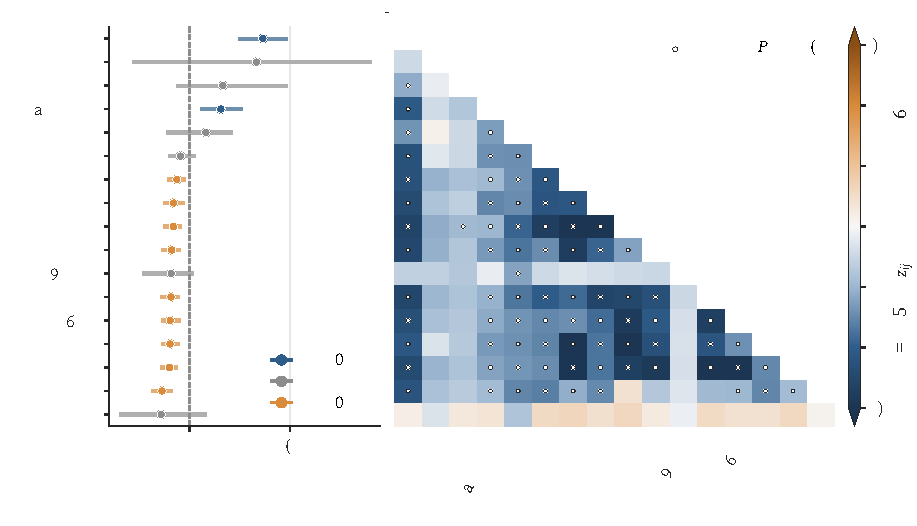
\includegraphics[width=\linewidth]{images/no1/P1_F06_领域边际效应与交互网络.pdf}
\caption{参考配比处的领域方向边际收益（a）与两两领域交互（b）}
\label{fig:p1_effects}
\end{figure}

式~\eqref{eq:p1_effect} 只描述 $\boldsymbol p_{\mathrm{ref}}$ 附近的一阶方向。为考察其是否依赖起点，在全部 512 个训练配方上做“局部替换”：按比例压缩其余 16 域、向目标领域转入 $2\%$ 份额，计算 13 域平均 Loss 的降低量（图~\ref{fig:p1_replace}）。技术对话、商务邮件与数学推理的中位降低量分别为 $0.107$、$0.097$ 和 $0.066$，技术对话与数学推理在 $91\%$ 的起点上有利；而哲学论文的有利占比只有 $52\%$，其效应不稳定。更重要的是，\textbf{17 个领域中有 14 个的增配收益与原有份额负相关}（Spearman 系数 $-0.26$ 至 $-0.69$，技术对话为 $-0.66$），呈现清晰的边际收益递减——这与数据混合律\cite{ye2025datamixinglaws,liu2025regmix}中“小领域少量增配收益最大”的经验一致。

\begin{figure}[htbp]
\centering
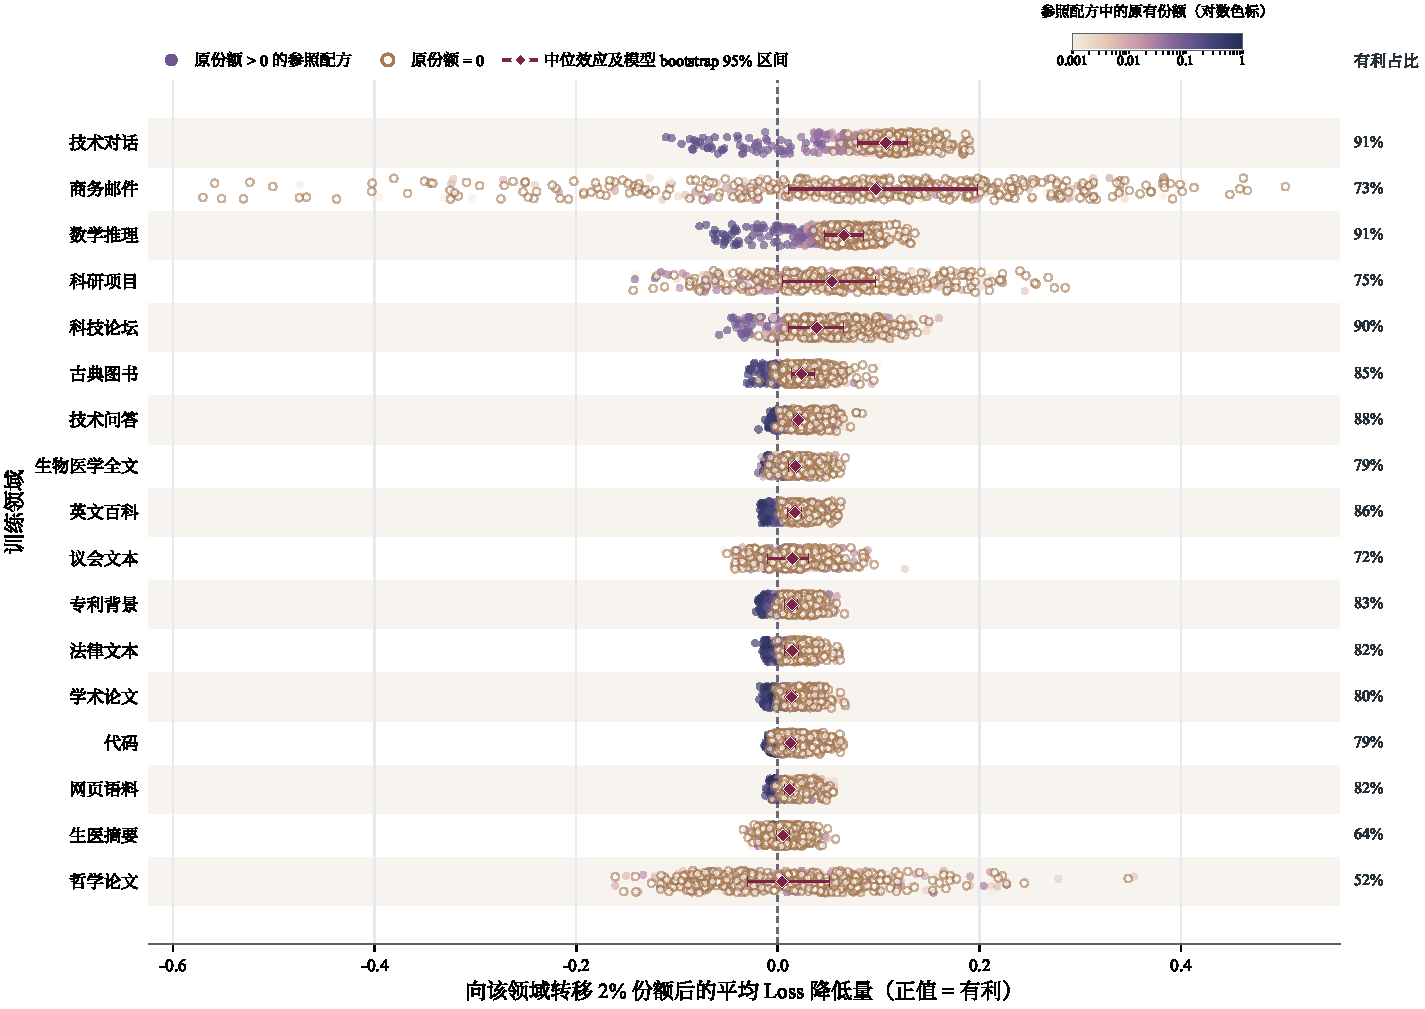
\includegraphics[width=\linewidth]{images/no1/P1_F08_领域局部替换效应.pdf}
\caption{512 个训练配方上转入 $2\%$ 份额的局部 Loss 降低量}
\label{fig:p1_replace}
\end{figure}

\subsubsection{领域组合：互补为主，未见稳定替代}

对 136 个交互系数做 500 次训练行 bootstrap（图~\ref{fig:p1_effects}(b)）。其中 $75$ 对的 95\% 区间完全小于 0，是\textbf{稳定互补}关系；有 15 对点估计为正（替代方向），但\textbf{没有一对}的区间完全大于 0。互补最强的组合集中在“稀缺小领域 × 其他领域”，例如科研项目—技术对话、技术对话—科技论坛、数学推理—技术对话、生物医学全文—科技论坛。这表明：在当前实验范围内，不同领域的数据主要是\textbf{互补品}而非替代品，混合多样化领域比集中投入单一领域更有效。

领域质量 $q_m$ 与边际收益 $E_i$ 的 Spearman、Kendall 系数分别为 $-0.143$、$-0.105$，二者没有正向单调关系：\textbf{质量高的领域不一定是最该增配的领域}。静态质量与动态配比收益是两个不同维度，这为问题二把质量与配比作为两条独立通道写入标度律提供了依据。

\subsubsection{支持域约束下的近优配比}

13 个验证域的 Loss 尺度不同，直接平均会让高波动领域主导目标。取训练集中第 $k$ 个验证域 Loss 的四分位距 $s_k$ 作尺度，定义综合目标
\begin{equation}
J(\boldsymbol p)=\frac1{13}\sum_{k=1}^{13}\frac{\widehat L_k(\boldsymbol p)}{s_k}.
\label{eq:p1_J}
\end{equation}
二阶响应面只在训练配方附近可靠，远离实验范围的“最优解”没有意义。令 $u_i$ 为训练配方中第 $i$ 个份额的 $99\%$ 分位，$\boldsymbol\sigma_p$ 为份额标准差，候选配比到训练集的标准化最近距离为 $d(\boldsymbol p)=\min_r\|(\boldsymbol p-\boldsymbol p_r)/\boldsymbol\sigma_p\|_2$，支持半径 $R_s$ 取训练点最近邻距离的 $99\%$ 分位。于是配比优化模型为
\begin{equation}
\min_{\boldsymbol p}\ J(\boldsymbol p)\qquad
\text{s.t.}\quad p_i\ge0,\quad \sum_{i=1}^{17}p_i=1,\quad p_i\le u_i,\quad d(\boldsymbol p)\le R_s .
\label{eq:p1_opt}
\end{equation}
以 30 个训练配方及其凸组合为起点做 SLSQP 求解，并用 $10000$ 个随机可行点做反证检查；在 200 次训练行 bootstrap 中重新拟合并重新优化，得到各份额的不确定区间。

\begin{table}[htbp]
\centering
\small
\caption{近优配比 $\boldsymbol p^\star$ 与参考配比 $\boldsymbol p_{\mathrm{ref}}$ 的对比（单位：\%）}
\label{tab:p1_pstar}
\begin{tabular}{lrrrl}
\toprule
领域 & $\boldsymbol p_{\mathrm{ref}}$ & $\boldsymbol p^\star$ & bootstrap 95\% 区间 & 调整方向 \\
\midrule
专利背景（USPTO） & 7.56 & 24.19 & [0.00, 55.61] & 承接份额 \\
生医摘要（PubMed Abs.） & 6.62 & 18.91 & [0.00, 53.09] & 承接份额 \\
技术问答（StackExchange） & 9.94 & 14.91 & [0.00, 51.08] & 增配 \\
议会文本（Europarl） & 1.27 & 10.38 & [0.00, 10.38] & 增配至上界 \\
科技论坛（HackerNews） & 1.17 & 7.15 & [0.00, 11.11] & 增配 \\
哲学论文（PhilPapers） & 0.55 & 4.88 & [0.00, 4.88] & 增配至上界 \\
技术对话（Ubuntu IRC） & 1.96 & 3.40 & [0.00, 16.98] & 增配 \\
商务邮件（Enron） & 0.22 & 2.09 & [0.00, 2.40] & 增配至近上界 \\
\midrule
生物医学全文、学术论文、代码、法律 & 43.43 & 0.00 & — & 压缩至 0 \\
网页语料（Pile-CC） & 11.95 & 3.55 & [0.00, 27.52] & 大幅压缩 \\
\bottomrule
\end{tabular}
\end{table}

结果见表~\ref{tab:p1_pstar} 与图~\ref{fig:p1_pstar}。近优配比的目标值为 $J(\boldsymbol p^\star)=4.765$，优于 $10000$ 个随机可行点中的最好值 $5.207$；约束回代的份额和误差为 $0$、上界违反量 $1.3\times10^{-14}$，支持距离恰好等于支持半径（$4.330$），即支持域约束\textbf{起作用}。优化的结构性规律非常清楚：

\begin{enumerate}
\item \textbf{压缩边际收益为负的大领域}：生物医学全文、学术论文、代码、法律四域由合计 $43.4\%$ 压缩至 0，网页语料由 $12.0\%$ 压缩至 $3.6\%$，这五个领域均属图~\ref{fig:p1_effects}(a) 中区间显著为负的九个领域；
\item \textbf{把稀缺的小领域推到经验上界}：议会文本、哲学论文触及上界，商务邮件接近上界，科技论坛增至上界的约 2/3——受限于实验中这些领域从未被大量使用，模型不敢把份额推得更远；
\item \textbf{由专利背景与生医摘要承接剩余份额}：它们在参考配比处的一阶边际收益虽为负，却与多个小领域存在稳定互补（如专利背景—科技论坛），说明份额调整由交互项而非一阶边际主导，二者是“承载”小领域收益的载体领域。
\end{enumerate}

需要说明的是，各份额的 bootstrap 区间较宽、多数领域有落到零的可能，且最优的 5 个起点目标值相对离散度为 $1.6\%$。因此 $\boldsymbol p^\star$ 应理解为“当前实验支持的\textbf{近优配比族}的代表”，其结构性方向（压缩大领域、增配稀缺领域）比单个份额的精确数值更可靠。

\begin{figure}[htbp]
\centering
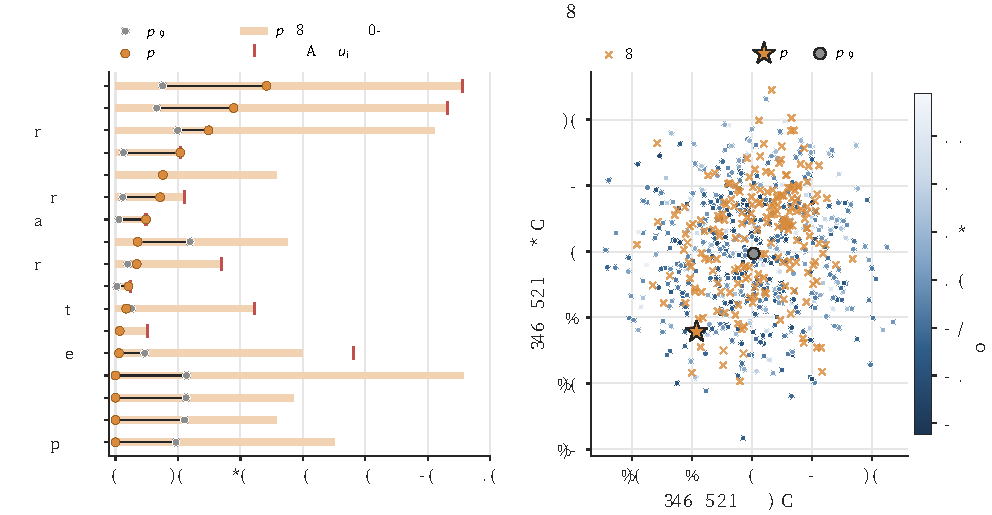
\includegraphics[width=\linewidth]{images/no1/P1_F07_组成空间近优配比与不确定性.pdf}
\caption{近优配比相对参考配比的调整及其不确定性}
\label{fig:p1_pstar}
\end{figure}

\subsubsection{近优配比的参数敏感性}

分别把支持半径分位、份额上界分位由 $99\%$ 收紧到 $97.5\%$、$95\%$，把 Ridge 正则强度改为 $0.5\alpha^*$、$2\alpha^*$，每个情景都重新做 30 起点优化（图~\ref{fig:p1_sens}）。正则强度扰动下，配比的 $L_1$ 变化仅 $2.8$、$3.9$ 个百分点，目标值几乎不变（$<0.02\%$）；而收紧支持半径至 $95\%$ 使配比变化 $20.1$ 个百分点、目标上升 $2.6\%$，收紧份额上界至 $95\%$ 使配比变化 $61.4$ 个百分点、目标上升 $3.4\%$。结论是：\textbf{近优配比对模型估计稳健，对“允许偏离实验范围多远”敏感}，扩大配比实验的覆盖范围是进一步提升配比收益的关键。

\begin{figure}[htbp]
\centering
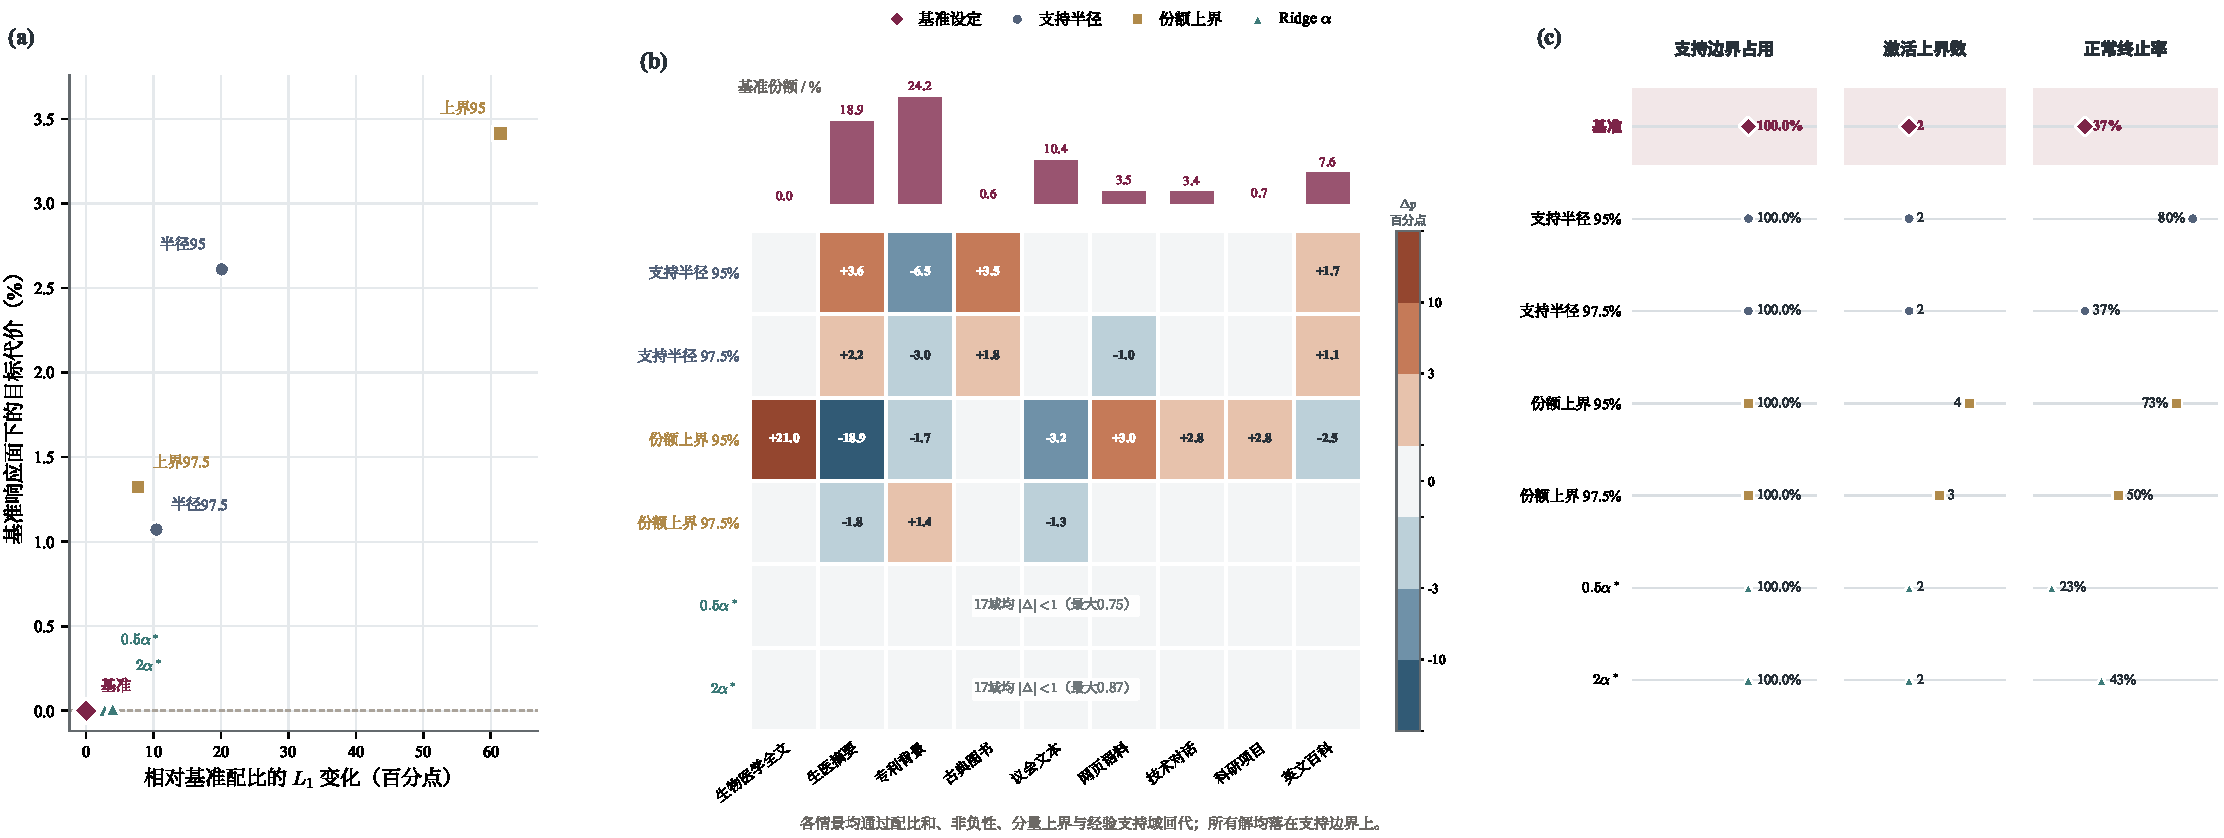
\includegraphics[width=\linewidth]{images/no1/P1_F10_近优配比参数敏感性.pdf}
\caption{近优配比对支持域、份额上界与正则强度的敏感性}
\label{fig:p1_sens}
\end{figure}

\subsection{问题一小结}

\begin{conclusionbox}
\textbf{问题一主要结论}
\begin{enumerate}
\item 构建“同向化—五语义块—稳定 CRITIC—Huber 冲突消解”质量评价模型，得到 26.1 万条独立记录的样本级与领域级质量：C4（$0.619$）$>$ CommonCrawl（$0.608$）$>$ arXiv（$0.569$）$>$ StackExchange（$0.561$）$>$ Book（$0.510$）$>$ Wikipedia（$0.507$）$>$ GitHub（$0.430$）；聚合规则扰动下七域排序 Kendall 系数最低为 $0.81$。
\item 显著冲突率为 $3.17\%$，其中 $93.4\%$ 的冲突以“结构充分”块为短板，成因是形式指标与内容指标的测量对象不同；这一结论在以扩展集为主体的 arXiv、GitHub 两域同样成立。抽样集与全量数据的域级质量一致（KS 距离 $\le0.025$），仅 arXiv 高分尾部存在差异。
\item 二阶 Scheff\'e--Ridge 混料模型在 1M、60M、1B 实测检验集上的 Spearman 系数为 $0.858$、$0.870$、$0.850$；技术对话与数学推理增配收益显著为正，领域间以互补为主（75 对稳定互补、0 对稳定替代）。近优配比压缩生物医学全文、学术论文、代码、法律等大领域，增配稀缺的对话、论坛、议会与哲学文本。
\item 向问题二输出：基线质量 $Q_0=\boldsymbol p_{\mathrm{ref}}^{\mathsf T}\boldsymbol q=0.5390$，参考配比 $\boldsymbol p_{\mathrm{ref}}$，近优配比 $\boldsymbol p^\star$，以及标准化配比响应 $R(\boldsymbol p)$（见式~\eqref{eq:p2_R}）。
\end{enumerate}
\end{conclusionbox}
